%\documentclass{article}
%\usepackage{graphicx,subfigure}
%\begin{document}

\begin{figure}[!h]
  \centering
  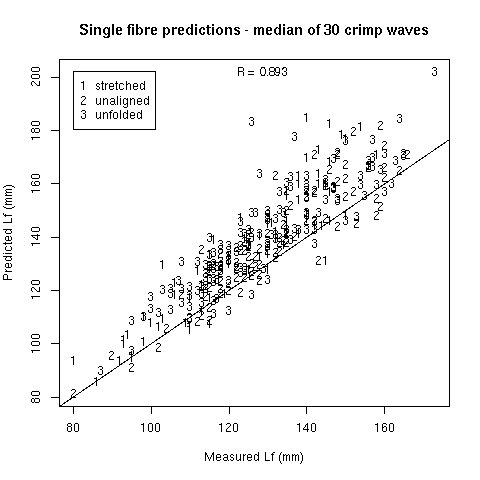
\includegraphics[width=1.1\textwidth]{figsfpredlffibre.png}
% original is 15fibrepredlfmedian.png
  \caption{Plot of measured fibre length against predicted mean fibre length for 315 individual fibres using Method 2 with predictions based on measurement of wavelength and amplitude by the SF technique, and crimps per staple calculated using relaxed fibre length instead of staple length. Fibre lengths for the unfolded crimp type wools were adjusted for the effect of twist at the points of inflection using $H = 0.5 * amplitude$ and $R = 0.10 mm$ in the prediction equations }
  \label{fig:sfpredlffibre}
\end{figure}

%\end{document}

